\documentclass[english, 11pt]{article}
\usepackage{notes}

% Uncomment these for a different family of fonts
% \usepackage{cmbright}
% \renewcommand{\sfdefault}{cmss}
% \renewcommand{\familydefault}{\sfdefault}

\newcommand{\thiscoursecode}{[730] (Deep Learning)}
\newcommand{\thiscoursename}{Albert Garcia}
\newcommand{\thisprof}{Vincent Vanhoucke}
\newcommand{\me}{Albert García}
\newcommand{\thisterm}{(Winter) 2016}
\newcommand{\website}{https://www.udacity.com/course/deep-learning--ud730}

% Headers
\chead{\thiscoursename \ Course Notes}
\lhead{\thisterm}


%%%%%% TITLE %%%%%%
\newcommand{\notefront} {
\pagenumbering{roman}
\begin{center}

{\ttfamily \url{\website}} {\small}

\textbf{\Huge{\noun{\thiscoursecode}}}{\Huge \par}

{\large{\noun{\thiscoursename}}}\\ \vspace{0.1in}

  {\noun \thisprof} \ $\bullet$ \ {\noun \thisterm} \ $\bullet$ \ {\noun {Udacity -- Google Research}} \\

  \end{center}
  }

% Begin Document
\begin{document}

  % Notes front
  \notefront
  % Table of Contents and List of Figures
  \tocandfigures
  % Abstract
  \doabstract{These notes are intended as a resource for myself; past, present, or future students of this course, and anyone interested in the material. The goal is to provide an end-to-end resource that covers all material discussed in the course displayed in an organized manner. If you spot any errors or would like to contribute, please contact me.}

	\section{Machine Learning to Deep Learning}

	\subsection{Linear Model}

	The most simple linear model that allows us to make predictions is represented by the following equation:
	\begin{align*}
		wx + b = y\,,
	\end{align*}

	where $w$ is the weights matrix, $b$ is the bias vector, $x$ is the matrix corresponding to the values of the sample to be clasified, and $y$ is the output or scores vector -- which has as many elements as classes can be classified. The training will change the values of the weights and biases to tune the prediction system so that for each input $x$ its correct class is predicted in $y$.

	\subsection{Softmax}

	The way to turn scores (also known as \emph{logits}) into probabilities is to use a \emph{softmax} function $S$ and apply it to all the elements of the classifier output vector $Y$. Assuming that the output of the classifier has $n$ dimensions, the softmax function is defined as follows

	\begin{align*}
		S(y_i) = \displaystyle\frac{e^{y_i}}{\displaystyle\sum_{j=0}^{n}e^{y_j}}\,.
	\end{align*}

	There are two important remarks about this softmax function. On the one hand, if the magnitude of the scores increases significantly, the probabilities get close to either $0$ or $1$. On the other hand, if the magnitude of the scores decreases, the probabilities tend to get close to the uniform distribution. In other words, increasing the magnitude of the classifier output makes the system more confident about the decision once softmax is applied and vice-versa (see Figure \ref{fig:softmax}). For machine learning systems, we would like to progressively turn the system from unsure to confident.

	\begin{figure}[!hbt]
		\centering
		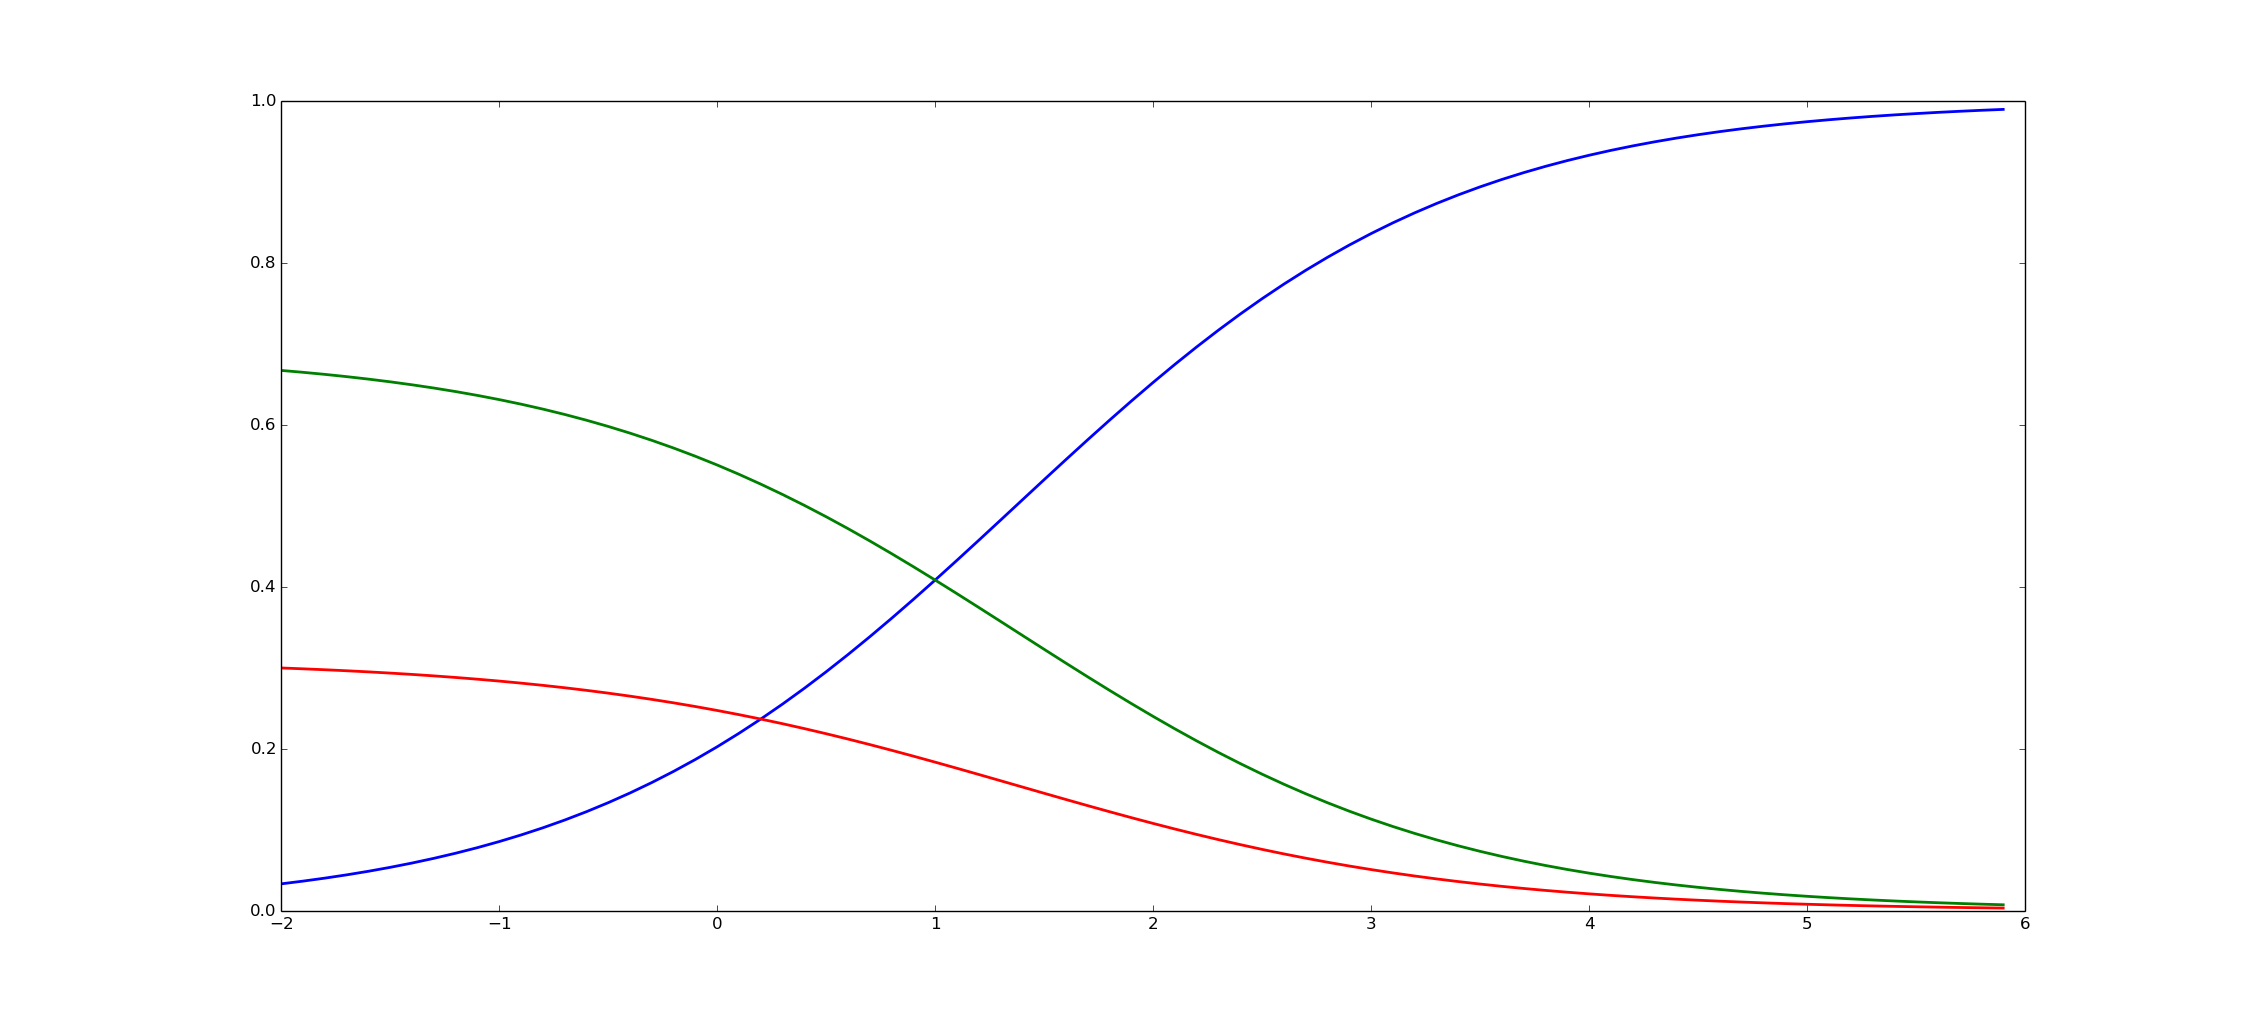
\includegraphics[width=0.5\linewidth]{l1/figures/softmax_output}
		\caption{Softmax outputs as the score of class $x$, in blue, increases.}
		\label{fig:softmax}
	\end{figure}

	\subsection{One-Hot Encoding}

	We need a way to represent class labels mathematically. We can use some sort of \emph{one-hot encoding} for that, representing each label with a vector that has as many elements as class labels our system is able to classify. Each one-hot class vector will have a $1$ at the position of the corresponding class, and the rest of the elements will be $0$.

	\begin{table}[!hbt]
		\centering
		\begin{tabular}{c|cccc}
			a & 0 & 0 & 0 & 1\\
			b & 0 & 0 & 1 & 0\\
			c & 1 & 0 & 0 & 0\\
			d & 0 & 1 & 0 & 0\\
		\end{tabular}
		\caption{One-hot encoding example vectors for four classes $a$, $b$, $c$, and $d$.}
	\end{table}

By doing this, we can map the classifier output probability provided by softmax to the appropriate class label following a likeness criteria. For instance, for the output probability vector $S(y)=\begin{bmatrix} 0.7 & 0.0 & 0.1 & 0.2\\ \end{bmatrix}$, and the one-hot encoding example shown previously, the most likely class is $c$.

	This approach works well for most of the cases, but in some situations we can have a vast number of classes so that we end up having huge class vectors with almost all positions filled up with zeroes. This turns out to be quite inefficient. However, using one-hot encoding provides us a way to determine how well our classifier is doing by comparing the probabilities vector provided by softmax and the correct class label one-hot encoded vector.

	\subsection{Cross Entropy}

	The natural way to measure the difference between two probability vectors is the \emph{cross-entropy} $D$. Given a probability vector from softmax $S(y)$, and a class label one-hot encoded vector $L$, their difference can be expressed as follows

	\begin{align*}
		D(S, L) = -\displaystyle\sum_{i=0}^{n}L_i \log(S_i)\,.
	\end{align*}

	\textbf{Be wary, $D(S, L) \neq D(L, S)$.}

	\subsection{Multinomial Logistic Classification}

	The setting that we have described throughout the previous sections takes an input $x$, which is turned into a logit $y$ by means of a linear model $wx + b = y$. Then, that logit is fed to a softmax layer $S(y)$ which converts those scores into probabilities. At last, the probabilities are compared to the different classes one-hot encoded labels using the cross-entropy function to determine the prediction. This setup is called multinomial logistic classification and it is represented by the following expression:

	\begin{align*}
		D(S(wx + b), L)
	\end{align*}

	\subsection{Minimizing Cross Entropy}

	In order to find the weights and biases that will produce low distances for the correct classes, e.g., $D(A,a)$, and high distances for incorrect ones, e.g., $D(A,b)$, we will minimize the loss $\zeta$ which is expressed as

	\begin{align*}
		\zeta(w, b) = \displaystyle\frac{1}{N}\displaystyle\sum_{i=0}^N D(S(wx_i+b),L_i)\,,
	\end{align*}

	where $N$ is the number of samples $x$ and labels $L$ in the training set. In other words, the loss is the average cross-entropy over the entire training set. This loss, is a function of multiple parameters: the weights and the biases. This function will be large in some areas and small in others. We will find the parameters that cause the loss to be the smallest as possible. By doing this, our problem is turned into a numerical optimization one.

	The simplest way to solve this problem is \emph{gradient descent}. This will take the derivative of the loss with respect to the parameters and follow that derivative by taking steps backwards until we get to a minimum, so the step will be $-\alpha\Delta\zeta(w, b)$. Figure \ref{fig:gradient-descent} represents this procedure for a simple loss function with two parameters.

	\begin{figure}[!hbt]
		\centering
		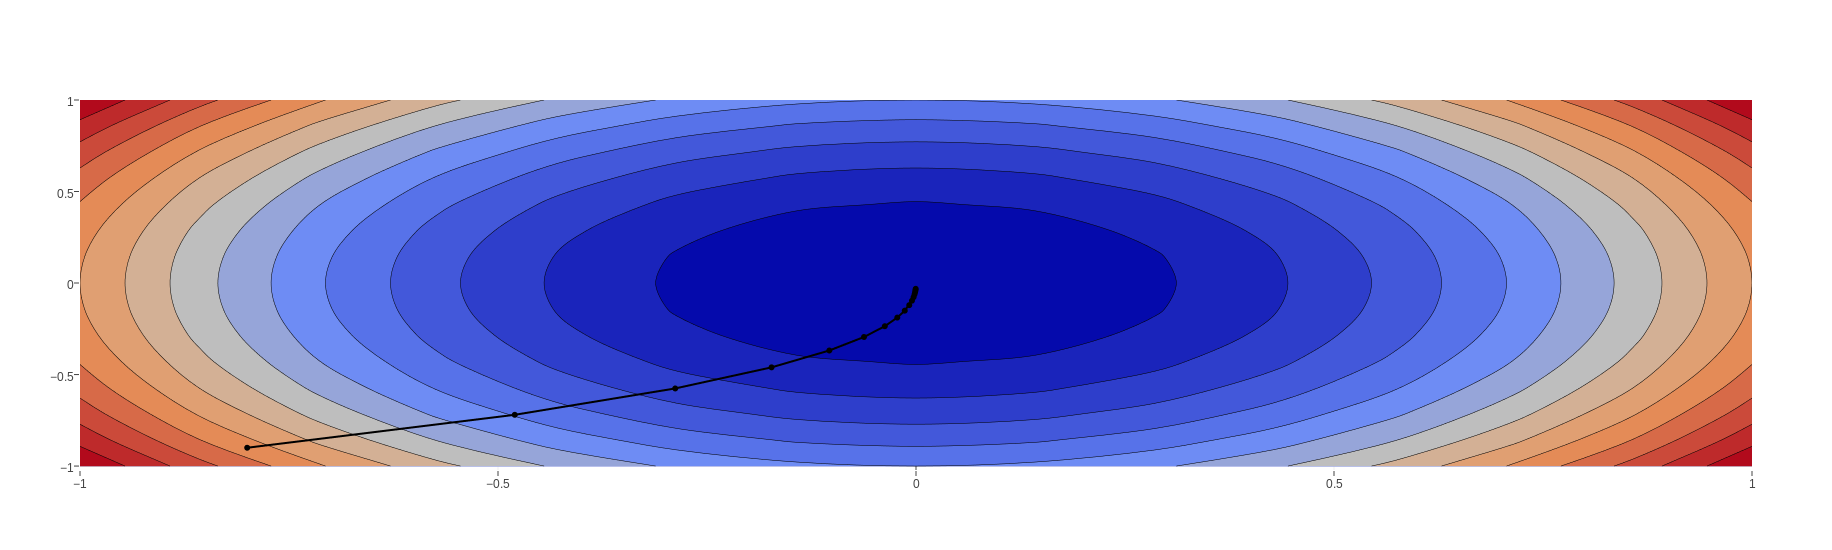
\includegraphics[width=\textwidth]{l1/figures/contour-scatter}
		\caption{Gradient descent from a larger area (red) to a smaller one (blue) taking steps following the derivative backwards (black) until the minimum is reached.}
		\label{fig:gradient-descent}
	\end{figure}
  %%%%%%%%%%%%%%%%%%%%%%%%%%%%%%%%%%%%%%%%%%%%%%%
  \end{document}
